\section{Durchführung}
\label{sec:Durchführung}
Der Versuchsaufbau gleicht prinzipell dem Aufbau für die Frauenhoferbeugung in Abbildung \ref{fig:frauenhofer}. Vor einem Spalt 
befindet sich ein He-Ne-Laser $\lambda=\SI{633}{\nano\metre}$, welcher kohärentes Licht aussendet. Hinter dem Spalt befindet sich dann in 
recht großer Entfernung $L$ ein Photoelement, welches über ein Amperemeter die Intensität $I$ des gebeugten Lichts misst. Um die 
winkelabahängigkeit des Beugungsbildes ausmessen zu können, ist das Photoelement beweglich auf einer skalierten Schiene verbaut.
In Abbildung \ref{fig:aufbau} ist der Aufbau noch einmal skizziert.
\begin{figure}[H]
    \centering
    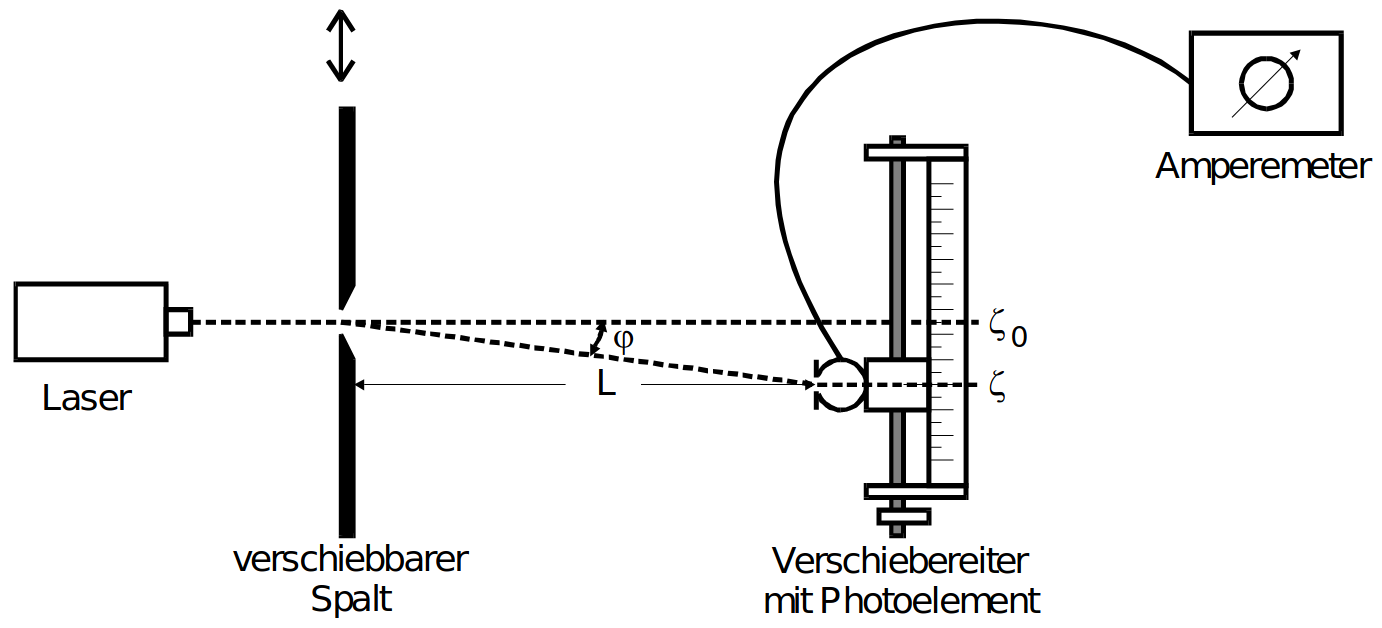
\includegraphics[scale = 0.35]{pictures/aufbau.png}
    \caption{Versuchsaufbau zur Messung der Intensitätsverteilung. \cite{AP01}}
    \label{fig:aufbau}
\end{figure}

\noindent
Vor Beginn der eigentlichen Messung muss der thermische Dunkelstrom notiert werden, den das Photoelement auch ohne Anschalten des Lasers
misst. DAfür wird der Versuchsraum möglichst abgedunkelt. Der Laser wird nun so justiert, dass das Licht durch den Spalt so auf das Photoelement trifft, 
dass sich das Hauptmaximum in der Mitte der Skala, d.h. $x=\SI{25}{\milli\metre}$, befindet und die Nebenmaxima in etwa die gleiche Intensität besitzen. 
\\\noindent
Dann werden zwei Messreihen 
mit jeweils $\num{60}$ Messungen durchgeführt, wobei in dem Bereich um das Hauptmaximum herrum $[\SI{20}{\milli\metre}-\SI{30}{\milli\metre}]$
in $\SI{0.5}{\milli\metre}$ Schritten und in dem restlichen Bereich von $[\SI{0}{\milli\metre}-\SI{50}{\milli\metre}]$ in $\SI{1}{\milli\metre}$
Schritten gemessen wird. In der ersten Messreihe wird ein Einzelspalt und in der zweiten ein Doppelspalt verwendet, wobei die 
Herstellerangaben bezügliche der Spaltbreite $b$ und des Spaltabstandes $s$ notiert werden. Zusätzlich zu den jeweils $\num{60}$ Messwerten 
wird noch der Abstand $L$ zwischen Spalt und Photoelement ausgemessen. 